% !TeX spellcheck = en_US
% !TEX root = ../thesis-example.tex
%

\begingroup
\let\cleardoublepage\clearpage

\chapter{Unitys' Monobehaviour Loop}
\label{app:engineloop}

The behavior of a Unity-initiated object is outlined by the following 
flowchart in \ref{fig:appendix:monoflow}, taken from Unitys' manual.

\begin{figure}[htb]
	\centering
	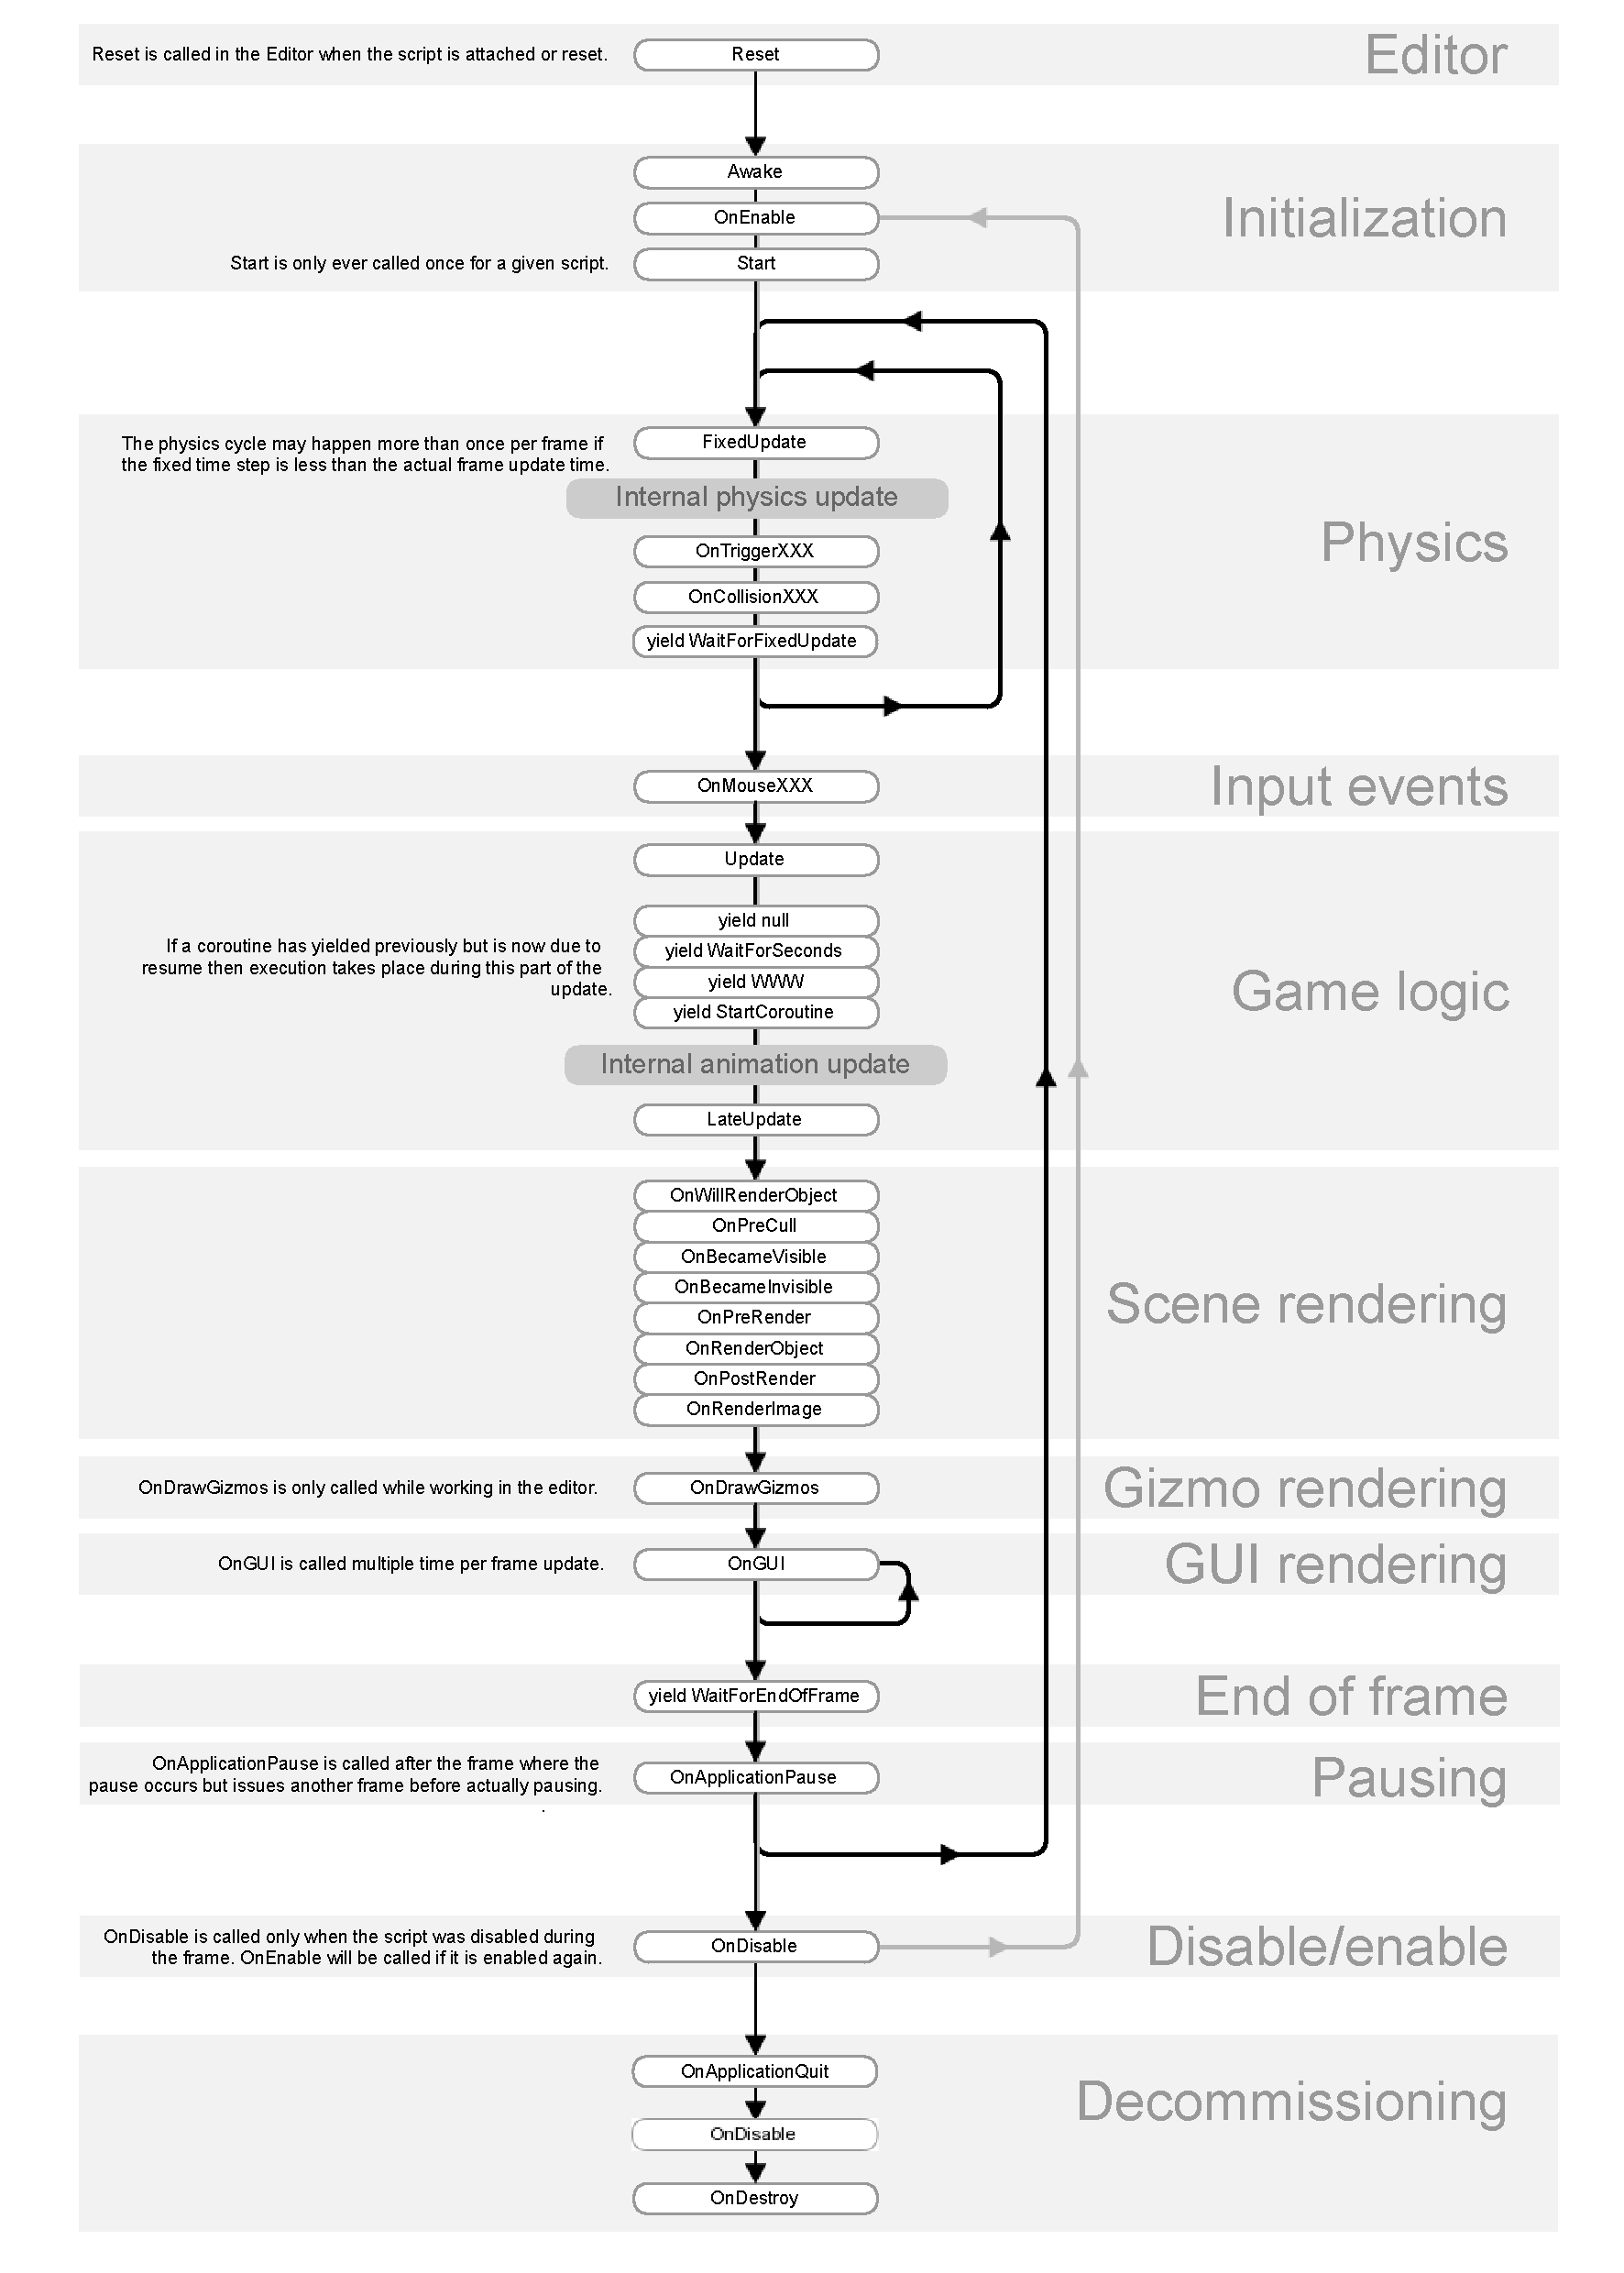
\includegraphics[width=0.85\textwidth]{_external/media/monobehaviour_flowchart2.pdf}
	\caption{Monobehaviour Flowchart}
	\label{fig:appendix:monoflow}
\end{figure}


\chapter{Simple Green Screen Setup}
\label{app:lightningsetup}

Building a green screen set is no easy task and takes a lot of careful 
consideration in light setup, background coloring and material used on set. 
\newline
Figure \ref{fig:appendix:gs-setup} shows a very simple and low-cost green 
screen setup after Foster et al. \cite{foster:greenscreen:2010}

\begin{figure}[htb]
	\centering
	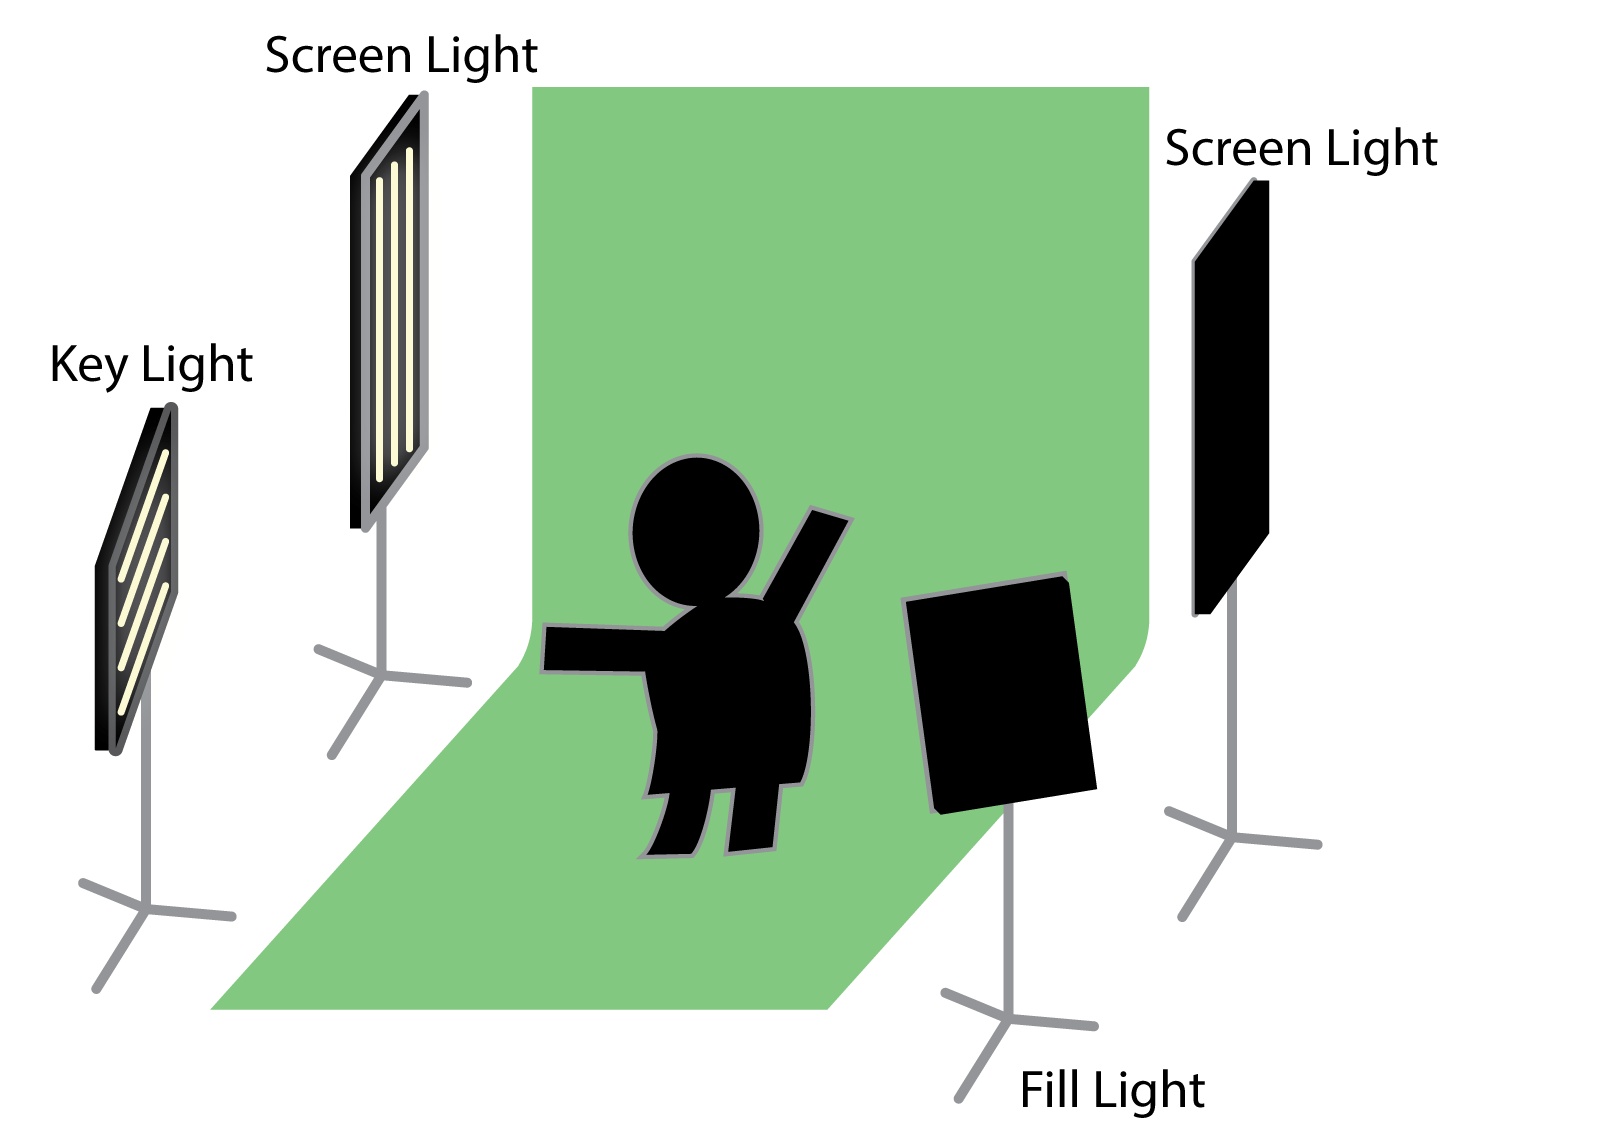
\includegraphics[width=\textwidth]{gfx/appendix/gs-setup.png}
	\caption{Basic green screen setup}
	\label{fig:appendix:gs-setup}
\end{figure}

\endgroup